\begin{comment}
    \begin{itemize}
        \item Unified discussion of results
        \item How they reinforce or contrast eachother
    \end{itemize}
\end{comment}

\subsection{Simulation Study}
To validate the variational model, we conduct a simulation study.
    As the problem of multivariate extremes is the estimation of the dependence
    structure of the extremes, we focus the simulation study on on estimation of
    the angular distribution.  The simulated data is generated from a finite
    mixture of projected gammas, at varying levels of dimensionality and number
    of mixture components.  For each simulation, for a \emph{training} dataset,
    \num{1000} replicates are sampled.  For each simulation, for a 
    \emph{testing} dataset, another \num{1000} replicates are sampled using
    the same distributional parameters.

To evaluate the fidelity of the variational implementation as compared to MCMC, 
    we use a the \emph{energy score} criterion \citep{gneiting2007}, which is a
    generalization of the \emph{continuous ranked probability score} to a
    multivariate setting.  This energy score criterion takes the form
    \[
      S_{\text{ES}}(P, \bm{x}) = \text{E}_p\left[g(\bm{X},\bm{x})\right] - 
        \frac{1}{2}\text{E}_p\left[g(\bm{X},\bm{X}^{\prime})\right]
    \]
    where $g$ is a kernel function, $\bm{x}$ is an observed value, and 
    $\bm{X},\bm{X}^{\prime}$ are posterior predictive replicates of $\bm{x}$.
    When energy score is used with an appropriate negative definite kernel 
    metric, it forms a \emph{proper} scoring rule. The specific negative 
    definite kernel we use is described in Prop.~3 of \cite{trubey:pg}.  Though 
    geodesic distance on $\mathbb{S}_{\infty}^{d-1}$ is computationally inefficient,
    for points on two different faces of $\mathbb{S}_{\infty}^{d-1}$,
    they find a computationally efficient upper bound on geodesic distance by 
    remembering that all faces are pairwise adjacent, and rotating one face into the
    same hyperplane as the other.  Then the kernel metric is the Euclidean distance
    between the first point, and the rotated second point.
    
    In Figure~\ref{fig:energyscore} we compare rise in energy score of the fitted
    model over a \emph{baseline} energy score.  This baseline energy score is so
    named because it is the energy score between a target dataset and another
    dataset from the same generating distribution.  A value of 0 is optimal.
    \makenote{add additional model for comparison}  Note displayed scores are 
    averaged over 10 iterations \makenote{rewrite}.

    \begin{figure}[ht]
        \centering
        \caption{Rise in energy score over baseline (Y) versus dimensionality (X),
            by number of latent mixture components in generating distribution
            \label{fig:energyscore}}
        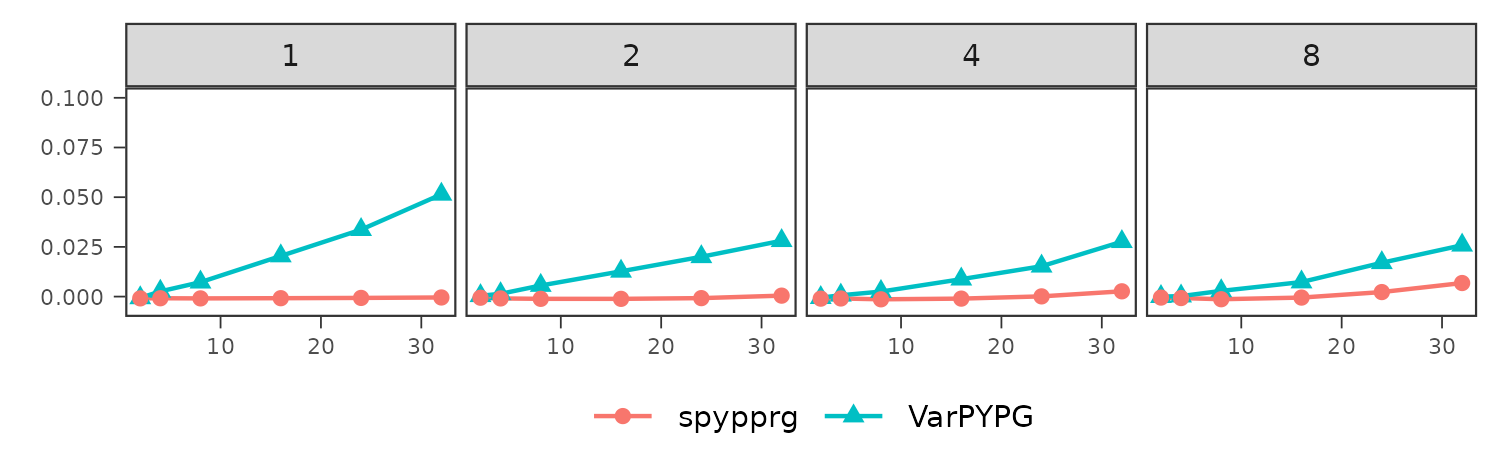
\includegraphics{./plots/energy_score}
    \end{figure}
    
    We see some minor loss in fidelity for the variational model as compared to 
    the MCMC model as is expected from the variational approximation.  With that
    said, the variational approximation is still quite good.

\subsection{SLOSH}

% EOF